% file: Generation_proc.tex
% date: 11/05/2020
% author: Enzo MEDINA emedina@enseirb-matmeca.fr
%         Mathieu BRASSART mbrassart001@enseirb-matmeca.fr
%         Léna HEREAU   phereau@enseir-matmeca.fr
%         Killian DIEU  kdieu@enseirb-matmeca.fr


\documentclass[a4paper]{article}

\usepackage[utf8]{inputenc}
\usepackage[french]{babel}
\usepackage{graphicx}
\graphicspath{{./rapport/}}
\usepackage{amsmath, amssymb}
\usepackage[left=3cm,right=3cm,top=2cm,bottom=2cm]{geometry}
\usepackage[dvipsnames]{xcolor}
\usepackage{tikz}
    \usetikzlibrary{positioning}
\usepackage{url}

\title{Projet S6: Génération Procédurale}
\author{Enzo Medina, Mathieu Brassart, Léna Herau, Killian Dieu}
\date{Mai 2021}

\usepackage[french]{babel}


\usepackage[utf8]{inputenc}
\usepackage[T1]{fontenc}
\usepackage{fullpage}
\usepackage{color}
\usepackage{listings}
\usepackage{algorithm}
\usepackage{algorithmic}

\renewcommand{\lstlistingname}{Algorithme}

\definecolor{codegreen}{RGB}{32, 124, 47}

\lstset{
  aboveskip=3mm,
  belowskip=-2mm,
  backgroundcolor=\color{white},
  basicstyle=\footnotesize,
  breakatwhitespace=false,
  breaklines=true,
  captionpos=b,
  commentstyle=\color{codegreen},
  deletekeywords={...},
  escapeinside={\%*}{*)},
  extendedchars=true,
  framexleftmargin=16pt,
  framextopmargin=3pt,
  framexbottommargin=6pt,
  frame=tb,
  keepspaces=true,
  keywordstyle=\color{blue},
  language=C,
  literate=
  {²}{{\textsuperscript{2}}}1
  {⁴}{{\textsuperscript{4}}}1
  {⁶}{{\textsuperscript{6}}}1
  {⁸}{{\textsuperscript{8}}}1
  {€}{{\euro{}}}1
  {é}{{\'e}}1
  {è}{{\`{e}}}1
  {ê}{{\^{e}}}1
  {ë}{{\¨{e}}}1
  {É}{{\'{E}}}1
  {Ê}{{\^{E}}}1
  {û}{{\^{u}}}1
  {ù}{{\`{u}}}1
  {â}{{\^{a}}}1
  {à}{{\`{a}}}1
  {á}{{\'{a}}}1
  {ã}{{\~{a}}}1
  {Á}{{\'{A}}}1
  {Â}{{\^{A}}}1
  {Ã}{{\~{A}}}1
  {ç}{{\c{c}}}1
  {Ç}{{\c{C}}}1
  {õ}{{\~{o}}}1
  {ó}{{\'{o}}}1
  {ô}{{\^{o}}}1
  {Õ}{{\~{O}}}1
  {Ó}{{\'{O}}}1
  {Ô}{{\^{O}}}1
  {î}{{\^{i}}}1
  {Î}{{\^{I}}}1
  {í}{{\'{i}}}1
  {Í}{{\~{Í}}}1,
  morekeywords={*,...},
  numbers=left,
  numbersep=10pt,
  numberstyle=\tiny\color{black},
  rulecolor=\color{black},
  showspaces=false,
  showstringspaces=false,
  showtabs=false,
  stepnumber=1,
  stringstyle=\color{black},
  tabsize=4,
  title=\lstname,
}


\begin{document}


\begin{titlepage}
    \begin{sffamily}
    \begin{center}
    
    ~\\[1.5cm]
    \textsc{\LARGE ENSEIRB-MATMECA}\\[1.5cm]
    
    \textsc{\Large Filière Informatique - 1ère année}\\[2cm]
    
    
        % Title
        \hrulefill \\[0.4cm]
    { \Huge \bfseries Rapport de projet S6 \\[0.4cm] }
    { \huge \bfseries Génération Procédurale \\[0.4cm] }
     \hrulefill \\[2cm]
     
     
\includegraphics[width=0.4\columnwidth]{logo-em.png} \\[1cm]
     
    % Authors
    \begin{minipage}{0.4\textwidth}
      \begin{flushleft} \large
         \emph{Auteurs :} \\
        Enzo MEDINA\\
        Mathieu BRASSART \\
        Léna HERAU \\
        Killian DIEU \\
      \end{flushleft}
    \end{minipage}
    \begin{minipage}{0.4\textwidth}
      \begin{flushright} \large
        \emph{Encadrants :} \\
        M. RENAULT\\
        M. SCHLICK \\
      \end{flushright}
    \end{minipage}
    
     ~\\[1.5cm]
    {\large 9 Mars 2021 — 21 Mai 2021}
    
    \end{center}
    \end{sffamily}
\end{titlepage}


\tableofcontents

\begin{figure}[hb]
    \centering ~\\[2cm]
    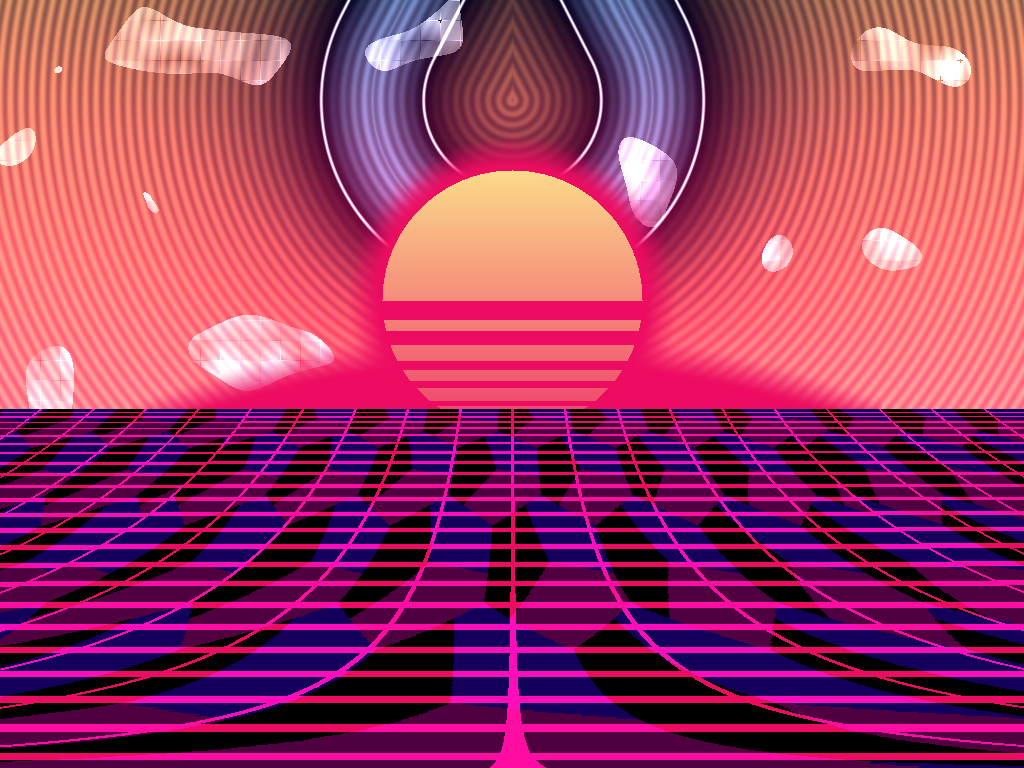
\includegraphics[width=0.8\columnwidth]{finalimage.png}
    \caption{Image finale du projet}
    \label{fig:finalimage}
\end{figure}

\newpage

\section{Introduction}

\paragraph{}
Le but de ce projet\cite{sujet} est de créer une bibliothèque de fonctions permettant de générer procéduralement des images, ainsi que de les modifier et de les composer entre elles. Ces fonctions devaient pouvoir être utilisées depuis une interface web (qui n'est pas au centre du projet) pour des exemples, et depuis un terminal grâce aux packages de node simulant un canvas.

\paragraph{}
Étant un projet de programmation fonctionnelle, d'importantes notions du cours\cite{cours} ont été gardées en tête pour établir une programmation dirigée par les fonctions, afin de composer aisément les fonctions, d'éviter des calculs inutiles ou redondants, et de profiter au maximum des outils mis à disposition spécifiquement par le langage Javascript choisi pour ce projet.

\paragraph{}
Dans une optique d'adaptabilité, les utilisateurs (et nous-mêmes) devaient finalement pouvoir ajouter des fonctions à cette bibliothèque de manière aisée, ainsi que profiter d'une documentation sur les fonctions implémentées. Nous avons de même conservé cette idée en tête tout le long du projet pour garder un code clair et une méthode d'ajout intuitive.



\section{Implémentation}
\paragraph{}
Le but de cette partie est de visualiser l'évolution du noyau du générateur d'images, de textures et de filtres. 

\subsection{Couleurs, textures et filtres}
\label{sec:colors}

\paragraph{}
Dès le début du projet, nous avons décidé de fixer précisément les représentations des différents objets utilisés dans la création d'images, afin que tous les ajouts à la bibliothèque lors du développement s'intègrent automatiquement. Dans la suite de ce rapport, nous nous référerons aux notions suivantes selon les définitions suivantes.

\paragraph{} 
Tout d'abord, une \textbf{couleur} est un quadruplet contenant respectivement les différentes composantes rouge, verte, bleue, et la transparence, alpha. Ce quadruplet dans notre code est un tableau de quatre éléments, \texttt{[R, G, B, A]}. Nous avons de plus fait un dictionnaire de couleurs prédéfinies afin de pouvoir en utiliser plus facilement.

\paragraph{}
Une \textbf{texture} est une fonction qui prend en entrée des paramètres et les coordonnées (x, y) d'un pixel, et renvoient une couleur. Appliquer une texture à tous les pixels d'une image crée donc l'image complète correspondant à cette texture. Elles commencent dans le code par le mot-clé \texttt{texture\_}.

\paragraph{}
Enfin, un \textbf{filtre} peut appartenir à deux catégories de fonctions, les filtres qui ne prennent qu'une seule image en entrée (appelés simplement filtres par la suite) et ceux qui en prennent deux (appelés \textbf{filtres doubles}). Dans les deux cas, ce sont des fonctions prenant en argument des paramètres et une ou deux images, et retournant une image complète en sortie. Ils commencent dans le code par les mots-clés \texttt{filter\_} et \texttt{dfilter\_}.

\paragraph{}
On peut ainsi appliquer successivement autant de filtres que l'on souhaite, à partir d'une image de base générée par une texture. C'est sur ce modèle (résumé dans la figure~\ref{fig:imagestructure}) que seront basés les générateurs d'images et arborescent développés plus bas. Deux fonctions sont ajoutées pour faire fonctionner le tout : \texttt{generateTexture} et \texttt{generateImage}, toutes deux définies dans la section~\ref{sec:node}.

\paragraph{}
Les différentes textures et filtres sont exportés puis rassemblés respectivement dans le même dictionnaire \texttt{TEXTURES} et \texttt{FILTERS} de la même façon que le dictionnaire \texttt{COLORS} contient l'ensemble des couleurs prédéfinies.

\begin{figure}[!ht]
    \centering
\begin{tikzpicture}[function/.style={rectangle, draw=black!70, fill=black!15, very thick, minimum size=7mm, rounded corners=1mm}, filter/.style={rectangle, draw=ForestGreen!60, fill=ForestGreen!15, very thick, minimum size=7mm, rounded corners=1mm}, texture/.style={rectangle, draw=RubineRed!60, fill=RubineRed!15, very thick, minimum size=7mm, rounded corners=1mm}, dots/.style={rectangle, draw=black!0, fill=black!5, very thick, minimum size=7mm, rounded corners=1mm}]

    % Nodes
    \node[texture]  (texture)                                   {Texture};
    \node[function] (gentexture)    [left=of texture]           {generateTexture()};
    \node[filter]   (filterdots)    [left=of gentexture]        {Filtre n°\dots};
    \node[filter]   (filter)        [left=of filterdots]        {Filtre n°1};
    \node[function] (genimage)      [left=of filter]            {generateImage()};
    
    % Lines ---------------
    \draw[->] (genimage.east) -- (filter.west);
    \draw[->] (filter.east) -- (filterdots.west);
    \draw[->] (filterdots.east) -- (gentexture.west);
    \draw[->] (gentexture.east) -- (texture.west);
    
\end{tikzpicture}
    \label{fig:imagestructure}
    \caption{Structure de création d'une image}
\end{figure}




\subsection{Transition de la currification aux dictionnaires}
\label{sec:curry}

\paragraph{}
Notre première approche dans la création des fonctions de la bibliothèque a été d'utiliser une currification complète. Ainsi, il fallait appeler un à un les paramètres des textures, jusqu'à appeler les coordonnées du pixel pour recevoir la couleur associée. Nous avons fait le choix tôt de mettre les coordonnées en dernière position dans toutes les fonctions, ainsi \texttt{generateTexture} pouvait rappeler la fonction jusqu'à ce que son type à l'itération suivante soit un tableau (une couleur), et alors itérer l'appel sur les pixels, ce qui évitait de recalculer les paramètres à chaque fois.

\paragraph{}
Cependant, cette implémentation posait deux problèmes. Le code ainsi écrit était extrêmement indenté (ou difficile à lire) car chaque paramètre rajoutait un niveau au bloc de la fonction. De plus, l'ordre des paramètres devait absolument être respecté, et aucun ne pouvait être omis. Pour palier à ces problèmes, il a été décidé d'utiliser des dictionnaires pour stocker les paramètres. Cependant, les coordonnées du pixel restent une fonction currifiée (de même que l'image en argument des filtres) pour accélérer l'exécution successive sans devoir recalculer les paramètres.

\paragraph{}
Chaque fonction dispose de plus de valeurs par défaut pour tous ses paramètres utiles, afin d'être exécutée depuis le navigateur pour un "cas d'exemple", et que chaque paramètre puisse être omis dans la déclaration. La taille par défaut s'adapte à celle du canvas, et les couleurs par défaut sont recherchées dans le dictionnaire de couleurs défini dans nos variables globales.



\subsection{Version web}
\label{sec:web}

\paragraph{}
La première interface que nous avons implémenté est celle utilisable depuis la page \texttt{public/index.html}. Pour la générer, il a été choisi d'utiliser le package \texttt{browserify} de Node.js, qui permet de rassembler l'intégralité de notre bibliothèque en un seul fichier de script appelé par la page web. A cet égard, le fichier \texttt{browser.js} sert à rassembler les fonctions utiles à l'interface, et à faire leur lien via l'objet \texttt{window} généré par le DOM.

\paragraph{}
Cette version nous a par ailleurs permis de générer des animations pour observer l'évolution temporelle de certains paramètres sur des fonctions. Cela a été particulièrement utile dans le cas des automates cellulaires (Jeu de la vie, Greenberg-Hastings, etc), où l'évolution dans les étapes permet de vérifier le bon fonctionnement des règles implémentées.



\subsection{Version node}
\label{sec:node}

\paragraph{}
Dans le cas de la version utilisable par ligne de commande, la fonction \texttt{require} et l'objet \texttt{exports} nous ont permis de séparer les fonctions et les filtres implémentés en divers fichiers indépendants. Un fichier \texttt{main\_func.js} se charge de récupérer toutes les fonctions générées, et de les classer dans des dictionnaires correspondant aux textures, filtres et filtres doubles. A l'intérieur se trouvent de plus les fonctions permettant de remplir un canvas, et le générateur arborescent détaillé plus loin. Le graphe de dépendance de cette version est représenté en figure~\ref{fig:dependancy}.

\begin{figure}[!ht]
    \centering
\begin{tikzpicture}[file/.style={rectangle, draw=black!70, fill=black!15, very thick, minimum size=7mm, rounded corners=1mm}, folder/.style={rectangle, draw=black!30, fill=black!5, very thick, minimum size=7mm, rounded corners=1mm}, mainfile/.style={rectangle, draw=RubineRed!60, fill=RubineRed!15, very thick, minimum size=7mm, rounded corners=1mm}, dots/.style={rectangle, draw=black!0, fill=black!5, very thick, minimum size=7mm, rounded corners=1mm}]

    % Nodes
    \node[file] (mainfunc)                                  {main\_func.js};
    \node[mainfile] (main)          [above right=of mainfunc]   {main.js};
    \node[mainfile] (browser)       [above left=of mainfunc]    {browser.js};
    \node[folder]   (textures)      [below right=of mainfunc]   {textures/};
    \node[folder]   (filters)       [below left=of mainfunc]    {filters/};
    \node[file]     (vars)          [below=of mainfunc]         {vars.js};
    \node[file]     (basictext)     [below=of textures]         {basic\_textures.js};
    \node[file]     (shapetext)     [below=of basictext]        {shape\_textures.js};
    \node[dots]     (dottext)       [right=of basictext]        {\dots};
    \node[file]     (basicfil)      [below=of filters]          {basic\_filters.js};
    \node[file]     (convofil)      [below=of basicfil]         {convolution\_filters.js};
    \node[dots]     (dotfil)        [left=of basicfil]          {\dots};
    
    % Lines ---------------
    \draw[->] (mainfunc.south) -- (vars.north);
    \draw[->] (browser.south east) -- (mainfunc.north west);
    \draw[->] (main.south west) -- (mainfunc.north east);
    \draw[->] (mainfunc.west) .. controls +(-2mm,0mm) and +(-0mm,15mm) .. (filters.north);
    \draw[->] (mainfunc.east) .. controls +(2mm,0mm) and +(-0mm,15mm) .. (textures.north);
    
    % Filters
    \draw[->] (filters.west) .. controls +(-2mm,0mm) and +(-10mm,15mm) .. (basicfil.west);
    \draw[->] (filters.west) .. controls +(-10mm,0mm) and +(-10mm,25mm) .. (convofil.west);
    \draw[->] (filters.west) .. controls +(-10mm,0mm) and +(0mm,5mm) .. (dotfil.north);
    \draw[->] (basicfil.east) .. controls +(0mm,0mm) and +(-5mm,-15mm) .. (vars.south);
    \draw[->] (convofil.east) .. controls +(0mm,0mm) and +(-5mm,-25mm) .. (vars.south);
    
    % Textures
    \draw[->] (textures.east) .. controls +(2mm,0mm) and +(10mm,15mm) .. (basictext.east);
    \draw[->] (textures.east) .. controls +(10mm,0mm) and +(10mm,25mm) .. (shapetext.east);
    \draw[->] (textures.east) .. controls +(10mm,0mm) and +(0mm,5mm) .. (dottext.north);
    \draw[->] (basictext.west) .. controls +(0mm,0mm) and +(5mm,-15mm) .. (vars.south);
    \draw[->] (shapetext.west) .. controls +(0mm,0mm) and +(5mm,-25mm) .. (vars.south);
    
\end{tikzpicture}
    \label{fig:dependancy}
    \caption{Graphe de dépendance du projet}
\end{figure}

\paragraph{}
Le fichier principal de cette version est \texttt{main.js}, se chargeant de générer une image à partir d'un fichier texte. Nous avons utilisé le package \texttt{fs}, pour "file system", pour récupérer les arguments en ligne de commande (voir \texttt{README.md} pour le format) et écrire dans un fichier l'image générée. 

\paragraph{}
Deux fonctions sont le coeur de notre projet. \textbf{generateTexture} se charge de parcourir tous les pixels d'une image avec hauteur et largeur définies, et d'interroger la texture passée en paramètre pour les remplir. \textbf{generateImage} récupère quant à elle ce résultat, pour les copier dans un canvas. On définit alors les canvas sur la page web et grâce au package \texttt{canvas} de node pour pouvoir les remplir.

\paragraph{}
Toutes les variables globales ont été stockées dans un fichier à part, modifiable par l'utilisateur, qui lui permet de spécifier la taille du canvas ou de définir des raccourcis pour des couleurs usuelles ("black" pour [0,0,0,255] par exemple). Certaines fonctions spécifiques sont elles aussi séparées du reste dans le fichier \texttt{textures/tools\_for\_textures.js}, puisqu'elles seront appelées dans plusieurs autres fichiers et ainsi n'ont pas besoin d'être redéfinies.

\paragraph{}
Notamment, un générateur aléatoire avec graine \textbf{getRandomIntSeed} y a été défini, puisque la fonction \texttt{random} de la bibliothèque Math est une des rares à ne pas fonctionner ainsi (merci à Mr Schlick\cite{seed} pour l'information). On utilise pour cela une fonction périodique à très haute fréquence, et on pioche le résultat à une abscisse définie par la graine.

\paragraph{}
Pour faciliter la création de motifs polygonaux, la fonction \textbf{isInShape} permet de renvoyer un booléen définissant si un point est à l'intérieur d'une forme polygonale définie par un ensemble de points. Cette fonction définit tout d'abord les parties concaves et convexes du polygone, et vérifie ensuite que le point passé en entrée appartient à la partie convexe tout en n'appartenant pas à la partie concave. Si l'une de ces conditions est fausse, le résultat est faux.



\subsection{Générateur arborescent}
\label{sec:arborescent}

\paragraph{}
Au sein de \texttt{main\_func.js} se trouve la fonction \textbf{generateArrayFromJson}, appelée à la fois dans la version node et la version web. Cette fonction permet de récupérer un objet JSON (obtenu via \texttt{JSON.parse} sur le fichier texte ou la textarea de la page web) et de la transformer en une image viable en agençant les textures, filtres et paramètres dans le bon ordre et en y insérant les fonctions de génération.

\paragraph{}
Fonctionnant récursivement grâce à la fonction \textbf{generateLevel}, l'algorithme parcourt les niveaux de l'objet JSON, en observe toutes les clés, et effectue une disjonction de cas pour savoir quelle marche à suivre suivant à quelle catégorie appartient la clé. Ces catégories sont générées grâce au nom des fonctions, qui sont conservées dans la propriété \texttt{name} malgré le renommage des exportations. Ainsi, le format défini au début du projet permet de séparer les fonctions démarrant par \texttt{texture\_} ou \texttt{filter\_}.

\paragraph{}
Si l'algorithme découvre une texture, alors il appelle \texttt{generateTexture} en utilisant la fonction dont le nom correspond dans le dictionnaire \texttt{TEXTURES}, et se rappelle récursivement sur la valeur de la clé pour générer les paramètres. S'il découvre un filtre, il peut interroger \texttt{FILTERS} et se rappelle récursivement deux fois. La première génère \textit{uniquement} les paramètres du filtre, et la seconde cherche quant à elle la texture associée. Un paramètre "argsOnly" permet de différencier ces cas.

\paragraph{}
Dans le cas d'un filtre double, il y a deux textures à trouver. Pour les différencier, un paramètre "search" permet de renvoyer uniquement le \textit{nom} de la première texture trouvée, afin d'être totalement indépendant de l'ordre des objets dans le dictionnaire lorsque la deuxième texture est observée. Celle-ci est définie comme "une texture trouvée dont le nom ne correspond pas à la valeur de \texttt{search}. Ce procédé pourrait être étendu à un tableau de valeurs dans le cas d'un filtre prenant $n$ textures comme arguments, en suivant le même modèle, mais nous n'avons pas eu le temps d'approfondir plus ce développement, toutefois nous avons fait une preuve de conception avec la fonction \texttt{galery} (voir figure~\ref{fig:galery}).

\begin{figure}
    \centering
    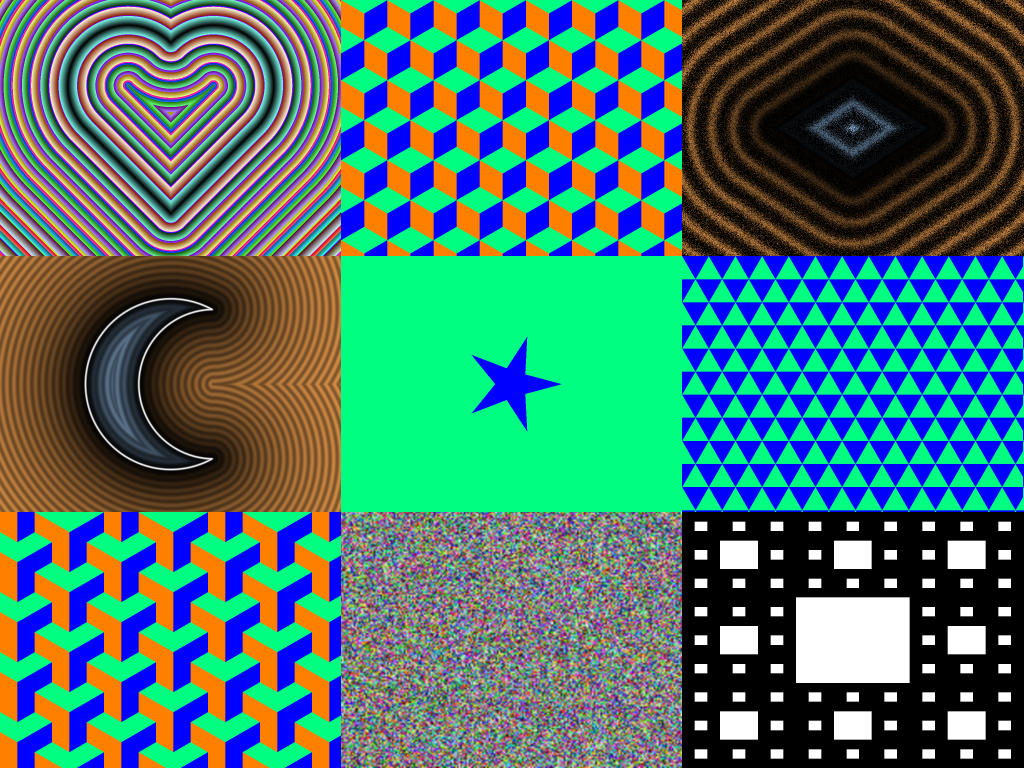
\includegraphics[width=0.6\columnwidth]{galery.png}
    \caption{Exemple de génération d'image avec le filtre galery}
    \label{fig:galery}
\end{figure}

\paragraph{}
Le mot-clé \texttt{dup\_} a été introduit pour permettre à deux fonctions au nom identique d'être appelées dans un filtre double, sans qu'il n'y ait d'écrasement des valeurs dans le cas de clés identiques. Un tel procédé aurait lui aussi pu être étendu en ajoutant un mot-clé plus global comme \texttt{dupX\_} avec $X$ un nombre, pour mettre en parallèle $n$ textures au nom identique.

\paragraph{}
Si une clé n'est pas reconnue, elle est considérée comme un paramètre, et ajoutée au dictionnaire actuel. Lorsque toutes les clés ont été parcourues, l'algorithme considère le dictionnaire actuel rempli, et le renvoie. Des cas spéciaux ont cependant été ajoutés pour permettre de remplacer la valeur de paramètres "color" par des chaînes de caractère, de même pour les règles des automates cellulaires.

\paragraph{}
Des aménagements à \textbf{generateTexture} ont finalement été effectués pour permettre d'utiliser des textures entières comme paramètres de couleur, en jouant sur le type (fonction ou tableau) du paramètre d'entrée.



\subsection{Documentation}
\label{sec:doc}

\paragraph{}
En raison de la faible importance de la documentation dans le sujet, très peu de temps y a été accordé. Ainsi, seuls les noms des fonctions utilisables, leur type (texture, filtre ou filtre double) et leurs paramètres éventuels sont répertoriés dans le fichier de documentation généré procéduralement.

\paragraph{}
Pour ce faire, les noms des fonctions sont récupérés dans les listes définies à la section~\ref{sec:arborescent} et affichées selon leur appartenance. Cependant, si cette partie est automatiquement réalisée par l'algorithme, l'utilisateur doit tout de même rajouter manuellement dans le fichier \texttt{makedoc.js} les paramètres associées à sa fonction, dans un nouveau cas d'une grande boucle \texttt{switch}.



\section{Fonctions implémentées}
\paragraph{}
Le but de cette partie est d'établir le travail effectué sur les différents filtres et textures implémentés, mais aussi des quelques animations créées.

\subsection{Textures}
\label{sec:textures}

\paragraph{}
Les premières textures implémentées ont été le \textbf{bruit blanc} ainsi que la \textbf{texture monochromatique}, puis un \textbf{gradient} simple qui par la suite a été amélioré en un gradient à répétition et pouvant être orienté à volonté (voir figure~\ref{fig:noises}).

\paragraph{}
Les trois \textbf{pavages réguliers} du plan ont été ajoutés, ainsi que les huit \textbf{pavages semi-réguliers}\cite{regularTiling} (à motifs composés de polygones réguliers). Plusieurs pavages à motifs contenant d'autres polygones ont été ajoutés, nos fonctions utilisant des sections rectangulaires se répétant dans le plan à un décalage près ou à la couleur près, en essayant de restreindre au maximum la taille de cette zone. Ainsi, des pavages constitués de pentagones orientés ou proposant des illusions d'effet 3D ont été intégrées à notre bibliothèque (voir figure~\ref{fig:tilings}).

\begin{figure}
    \centering
    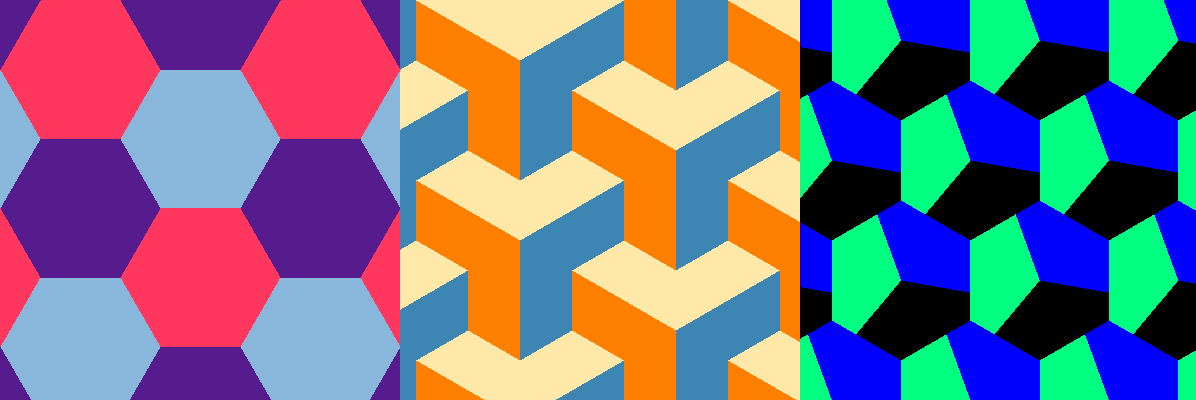
\includegraphics[width=0.8\columnwidth]{tilings.png}
    \caption{Exemples de pavages implémentés}
    \label{fig:tilings}
\end{figure}

\paragraph{}
Le bruit de Perlin et le bruit blanc limité en fréquence ont été implémentés eux aussi (voir figure~\ref{fig:noises}). Ces deux bruits se basent sur la notion d'interpolation de valeurs. En ce qui concerne le bruit blanc limité en fréquence, un nombre défini de pixel ont une couleur aléatoire. Les autres pixels, quant à eux, ont une couleur dépendante des un à quatre pixels prédéfinis autour d'eux. La couleur du pixel est calculée en fonction de la distance avec les autres pixels : plus un pixel prédéfini est loin, moins sa couleur sera importante pour sa définition. En interpolant les distances dans la couleur des pixels, des gradients entre les pixels prédéfinis sont formés.

Dans le bruit de Perlin, on définit un nombre arbitraire de vecteurs, disposés de manière régulière. Grâce à ces vecteurs, on peut déterminer les produits scalaires des vecteurs alentours puis interpoler ces valeurs avec une fonction spécifique de lissage.


\begin{figure}
    \centering
    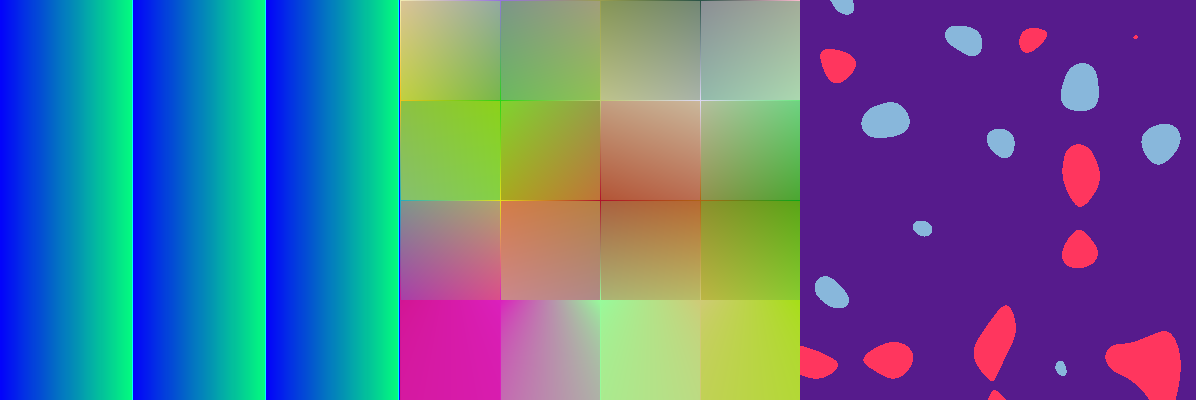
\includegraphics[width=0.8\columnwidth]{noises.png}
    \caption{Gradient, bruit blanc limité et bruit de Perlin}
    \label{fig:noises}
\end{figure}

\paragraph{}
Nous avons mis au point une fonction permettant de créer un polygone quelconque à partir des coordonnées des points le définissant (voir algorithme~\ref{algo:isInShape}), ce qui nous a permis de créer une fonction dessinant un \textbf{polygone régulier} en spécifiant le nombre de côté voulu. De même, les textures d'\textbf{étoiles à $N$ branches} et de \textbf{double étoile} ont pu être ajoutées. Cette fonction pourrait servir pour beaucoup d'autres formes, mais un de ses désavantages est qu'elle peut prendre beaucoup de temps de calcul, notamment lorsque la forme voulue a beaucoup de côtés ou simplement lorsqu'elle est concave (voir section~\ref{sec:node}). 

\begin{lstlisting}[caption ={Fonction déterminant l'appartenance d'un point à une forme}, label=algo:isInShape, float=h]
    fonction(points : tableau de points)
        Si longueur(points) < 3
            retourner fonction() {retourner faux;};
        Sinon
            Si les points ne sont pas définis dans le bon sens
                points = inverser(points);
            formes = []; // liste des formes à retirer pour obtenir une forme convexe
            [points', indices] = [];
            TantQue le nombre de formes est différent de l'appel précédent
                [points', indices] = retirerPointsConcaves(points);
                formes = ajouter(formes, retirerForme(points, indices));
                points = points';
            retourner fonction(x, y) 
                Si (x, y) appartient à points' Et n'appartient à aucune forme de formes
                    retourner vrai;
                Sinon 
                    retourner faux;
\end{lstlisting}

\paragraph{}
Nous nous sommes par la suite intéressés aux \textbf{automates cellulaires} tels que le feu de foret, le jeu de la vie\cite{goL}, Greenberg Hastings ou encore les automates élémentaires et cycliques en une seule dimension. Ces trois fonctions sont représentées (agrandies) dans la figure~\ref{fig:automates}. Les textures à étapes opèrent en se basant sur une fonction \texttt{getMooreNeighboorState} récupérant l'état des voisins de Moore\cite{moore} d'un pixel (au plus les huit voisins autour de lui), puis en la passant dans une méthode \texttt{reduce} afin d'assigner une constante de décision à ce pixel (par exemple, en connaissant le nombre de ses voisins "en vie"). Pour les \textbf{automates élémentaires}\cite{elemCellu}, plusieurs règles et conditions initiales ont été implémentées, ainsi que la façon de gérer ces règles facilement. Les utilisateurs peuvent donc ajouter de nouvelles règles pour enrichir la bibliothèque du projet de façon aisée.

\paragraph{}
Chaque génération d'automate cellulaire fonctionne de la même manière, aux règles d'évolution près. Tout d'abord, la situation initiale est générée, par aléatoire ou une fonction donnée. Ensuite, l'étape suivante est calculée grâce à une fonction \texttt{x\_nextStep} où $x$ représente le nom de l'automate. Après fin de calcul, l'automate se trouve dans l'état final, et est donc prêt à être représenté.

Petit point tout de même à souligner est la redondance de ces générations. En effet, il aurait été tout à fait possible de ne créer qu'une seule fonction génératrice et lui passer en paramètres deux fonctions: l'initialisation et le passage à l'étape suivante. Cet exemple est visible dans le cas des automates cellulaires à une dimension, où la règle choisie ainsi que la situation initiale sont données en paramètres. L'extension de cette forme à tous les automates cellulaires serait une bonne piste d'optimisation de ces générateurs de texture.

\begin{figure}
    \centering
    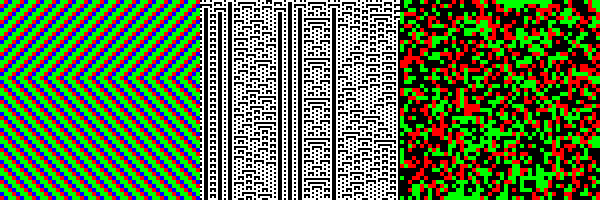
\includegraphics[width=0.8\columnwidth]{automates.png}
    \caption{Automates cellulaires (GreenbergHastings, 1D règle 73 et feu de forêt)}
    \label{fig:automates}
\end{figure}

\paragraph{}
Ensuite, les textures \textbf{fractales} ont été implémentées, le triangle de Sierpinski et le tapis de Sierpinski, où il suffit de définir le motif de profondeur $1$ puis les transitions d'une profondeur à la suivante, qui dépendent de la zone où se trouve le pixel. Ces fonctions opèrent récursivement sur le niveau de profondeur, en décidant à chaque niveau si le pixel concerné est dans l'une des multiples zones où un nouvel appel est nécessaire.

\paragraph{}
Enfin, nous avons fini par les textures à base de \textbf{distance signée}\cite{signedDistance}, où la couleur d'un pixel est définie en fonction de sa distance à la forme, qu'il soit à l'intérieur ou à l'extérieur de celle-ci. Ces textures peuvent prendre en argument une fonction qui définie la couleur par rapport à la distance (voir exemples en figure~\ref{fig:signed}), et sont parmi les plus modulables de la bibliothèque.

\begin{figure}
    \centering
    
\includegraphics[width=0.8\columnwidth]{signed.png}
    \caption{Exemples de textures à base de distance signée implémentées}
    \label{fig:signed}
\end{figure}

\paragraph{}
De nombreux paramètres ont été ajoutés aux fonctions de texture qui le permettaient, pour rendre le rendu personnalisable au maximum. Ainsi, toutes les textures ont les paramètres largeur, longueur, et ont leurs couleurs modifiables. Les textures non-régulières ont des paramètres de centrage ou de décalage, et toutes les textures orientables ont un angle réglable. Finalement, certaines textures (comme les distances signées) ont presque toutes leurs caractéristiques modifiables (avec trois tailles différentes, et des fonctions de couleur sélectionnables). D'autres paramètres sont disponibles individuellement sur certaines textures, car nous avons jugé moins utile de prendre le temps de les étendre à l'intégralité de nos fonctions, que d'utiliser ce temps à de meilleures fins.

\paragraph{}
Puisque les objets JSON ne reconnaissent pas les objets "fonction" de Javascript, il a fallu créer des bibliothèques de fonctions pré-définies pour les textures utilisant des fonctions personnalisées. Celles-ci se trouvent ainsi dans des boucles \texttt{switch}, accessibles par une chaîne de caractère (qui elle est reconnue par le JSON).

\subsection{Filtres}
\label{sec:filters}

Nous avons implémenté plusieurs catégories de filtres, avec tout d'abord les \textbf{filtres basiques} tels que la \textbf{translation} ou la \textbf{rotation} qui permettent d'appliquer un changement de coordonnées identique aux pixels de l'image. Ensuite les filtres de renversement de l'image, horizontalement et verticalement qui permettent respectivement d'inverser le haut avec le bas et la gauche avec la droite. Enfin dans cet ensemble, nous avons ajouté un filtre négatif qui inverse la couleur des pixels, un filtre de zoom qui permet d'agrandir une image sur une zone de l'image, un filtre qui remplace chaque couleur par son équivalent en teinte de gris et enfin un filtre qui permet de remplacer une couleur par une autre. Un aperçu de ces filtres se trouve en figure~\ref{fig:basicfil}

\begin{figure}
    \centering
    
\includegraphics[width=0.8\columnwidth]{basicfil.png}
    \caption{Agrandissement, inversion des couleurs et niveaux de gris}
    \label{fig:basicfil}
\end{figure}

\paragraph{}
Pour se rapprocher des filtres que proposerait un logiciel de manipulation d'image classique, nous avons implémenté deux systèmes de décomposition : un \textbf{séparateur en canaux RGB}, et un \textbf{séparateur en canaux HSL}\cite{rgb2hsl} (Teinte, Saturation, Luminosité). Une fois les canaux séparés, il devient aisé de les manipuler individuellement avant de les rassembler à nouveau, donnant naissance à des filtres de saturation, de rotation de teinte, de modification de \textbf{contraste}\cite{contrast} ou de luminosité (voir figure~\ref{fig:colors}).

\begin{figure}
    \centering
    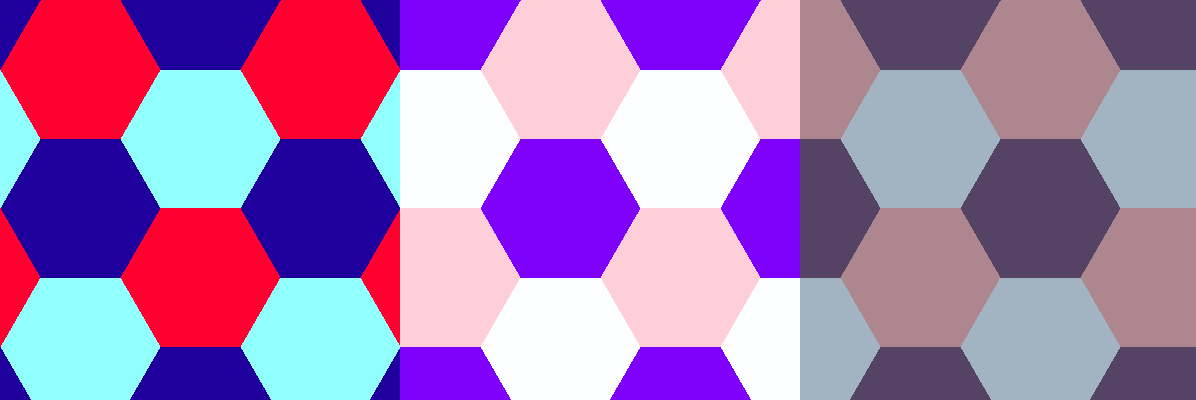
\includegraphics[width=0.8\columnwidth]{colors.png}
    \caption{Amélioration du contraste, de la luminosité, et diminution de la saturation}
    \label{fig:colors}
\end{figure}

\paragraph{}
L'implémentation des double filtres comprend les compositions d'images par convolution (voir figure~\ref{fig:compose}), définies par des opérations pixel à pixel entre deux images (addition, soustraction, différence, le plus ou le moins lumineux, ...) respectant la spécification SVG\cite{composition}. Des double filtres supplémentaires ont été ajoutées pour permettre de retrancher ou coller une image sur une autre, pour modéliser de la profondeur et simuler la présence de calques additifs et soustractifs (visibles dans la figure~\ref{fig:layers}).

\begin{figure}
    \centering
    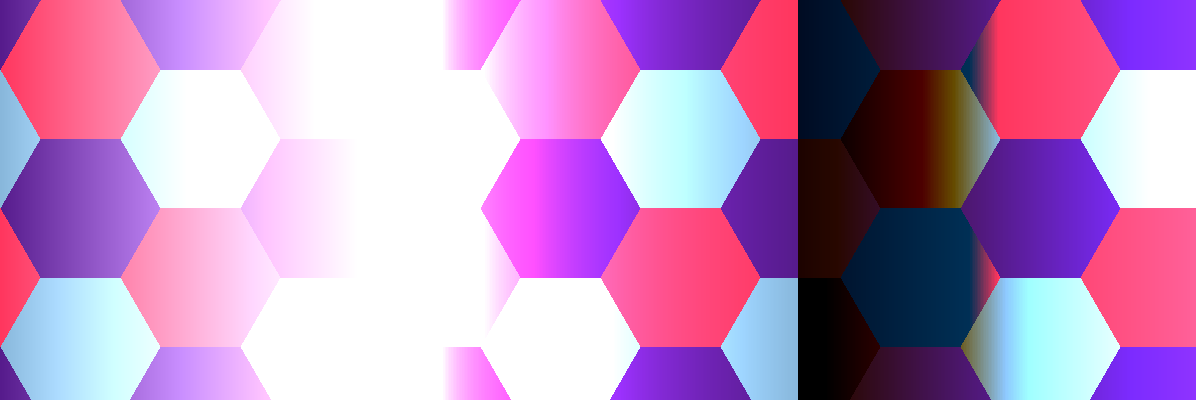
\includegraphics[width=0.8\columnwidth]{compose.png}
    \caption{Opérations "plus", "divide", "softlighten" entre un pavage et un gradient noir-blanc}
    \label{fig:compose}
\end{figure}

\begin{figure}
    \centering
    
\includegraphics[width=0.8\columnwidth]{layers.png}
    \caption{Filtres d'ajout et de retranchement d'un rectangle violet sur un rose.}
    \label{fig:layers}
\end{figure}

\paragraph{}
Les filtres se poursuivent par les \textbf{filtres de convolution} (voir figure~\ref{fig:convolution}), contenant plusieurs fonctions de flou et de détection des contours. Le premier flou implémenté est un flou simple où chaque pixel devient la moyenne des couleurs autour de lui dans un certain rayon en utilisant une distance de Manhattan, et dont les bords de l'image sont gérés de façon à ne faire la moyenne uniquement sur les pixels existants autour de lui. 

\begin{figure}
    \centering
    
\includegraphics[width=0.8\columnwidth]{convo.png}
    \caption{Filtres de convolution : Sobel, Canny, flou de boîte}
    \label{fig:convolution}
\end{figure}

\paragraph{}
Les suivants utilisent des \textbf{masques}, appliqués sur l'ensemble de l'image et un nombre de pixels constant. Cela signifie que la gestion des bords est plus complexe, et notre bibliothèque en implémente trois propositions : une gestion par extension, par enroulement ou par miroir. Nous avons ainsi implémenté un filtre de \textbf{flou gaussien} qui applique un masque gaussien (avec choix du rayon et de la déviation standard) sur l'ensemble de l'image, et un \textbf{flou de boite} semblable au flou simple mais différant dans deux domaines : ici, le rayon de convolution est constant, et c'est le voisinage de Moore qui est considéré (au lieu du voisinage de Von Neumann dans le flou simple).

\paragraph{}
Les filtres de convolution comprennent également les détections de contour par la méthode de \textbf{Sobel} ou la méthode de \textbf{Canny}. La première détecte les contours en attribuant le degré de différence qu'un pixel a avec son voisinage, alors que la méthode de Canny réduit d'abord le bruit de l'image passée en niveaux de gris, puis en récupère le gradient pour ne garder que les maximums locaux avant d'appliquer un filtre a hystérésis pour en récupérer seulement la partie épurée.

\textbf{}
Des filtres d'\textbf{amplification ou d'adoucissement des contours} ont aussi été implémentés, avec une fonction qui crée une bordure entre deux pixels lorsqu'ils sont différents selon une sensibilité, et un filtre d'adoucissement par la méthode gaussienne et selon une méthode linéaire.

\paragraph{}
Pour finir, un filtre de \textbf{transformation conforme} a été ajouté à notre bibliothèque de fonctions, permettant d'appliquer à tout les pixels de l'image une modification de coordonnées selon une transformation bijective. Des exemples avec les fonctions $x \mapsto x^2$, $x \mapsto \sqrt{x}$, ou des enroulements de l'image ont été ajoutés, et d'autres peuvent être greffés aisément au système. Pour chaque fonction, c'est sa réciproque qui est définie en amont (car son calcul serait trop lourd et n'est pas l'objet du projet) et est appliquée aux coordonnées d'un pixel pour savoir où se trouve son pixel antécédent.


\subsection{Animations}
\label{sec:animations}

\paragraph{}
Comme présenté par notre encadrant M. Schlick, nous avons implémenté des animations en s'inspirant du code proposé puis nous l'avons transformé en un générateur d'animations (\texttt{generateAnimation}) qui permet, comme pour les textures, de prendre en entrée une fonctions d'animations puis pour chaque coordonnées d'un pixel \texttt{(x, y)} et pour chaque instant \texttt{dt}, de renvoyer la couleur de ce pixel.

\paragraph{}
Pour commencer, nous avons implémenté des fonctions assez simples comme \texttt{chromaticCircle}, un cercle dont la couleur change au cours du temps, ce qui ne requiert que la définition d'une fonction périodique pour chaque composante de la couleur de remplissage. La fonction \texttt{add\_animation} permet quant à elle d'animer les textures de notre bibliothèque, ce qui se fait par des transformations sur les coordonnées. Pour simplifier ces animations, des fonctions de translation et de rotation dans le plan ont été implémentées.

\paragraph{}
Par la suite nous avons animé le pavage du Caire pour aller de la forme carrée au rectangle dans ses états limites. Un yin yang à également été animé, tournant sur lui-même. Ces animations sont produites de la même manière : à chaque instant un paramètre est changé d'un certain delta puis la fonction de texture est appelée avec ce paramètre. Ces essais nous ont permis de vérifier l'impact de nos paramètres et de corriger d'éventuels bugs.

\paragraph{}
Enfin vient l'animation des fonctions à états comme les automates cellulaires. Ces animations sont réalisées par la création d'un noeud contenant un état et l'appel fonction de transition vers l'état suivant. La création d'une fonction permettant la création infinie d'états était donc nécessaire, ce qui se résume par un noeud contenant l'état initial et l'appel gelé à la fonction générant l'état suivant.

\paragraph{}
Cela nous a permis de réaliser une fonction animant aléatoirement les textures de notre bibliothèque, mais aussi l'évolution du jeu de la vie, notamment avec des configurations de départ, le feu de foret, Greenberg Hastings et un effet de pluie. C'est par l'observation de ces résultats que la correction du comportement de nos automates a pu être attestée. Pour le jeu de la vie et Greenberg Hastings, on initialise différentes configurations spéciales pour un résultat intéressant comme par exemple le \texttt{gosper glider gun}, le premier motif de taille infinie découvert.

\paragraph{}
Cette partie du projet ne faisant pas partie des exigences mais ressortant de la proposition de notre encadrant, elle était intéressante à traiter, notamment pour les animations à états qui ont introduit la création infinie d'états. Cependant, les latences peuvent vite se ressentir puisque le Javascript n'est pas très adapté à cet usage.

\section{Tests}
\paragraph{}
Afin de tester certaines de nos fonctions nous avons utilisé le module \textbf{Jest}. Ce module permet par sa simplicité d'utilisation et sa modularité de créer des tests dans un dossier séparé dans différents fichiers. Notre module de test est découpé en deux suites majeures : une pour les textures et une pour les filtres. Chacun des tests dans ces suites se déroulent d'une manière similaire. Dans un premier temps, on calcule le résultat attendu de l'appel de la fonction que l'on teste; ici, on compare des images ou des automates cellulaires. Ensuite, on simule un canvas ou un automate cellulaire d'une taille prédéfinie ($3 \times 3$ ou $5 \times 5$ dans nos tests) et on lui applique la fonction testée. Enfin, on compare valeur à valeur l'égalité de l'objet retourné par la fonction et de l'objet attendu.

\subsection{Textures}
\label{texturestest}
\paragraph{}
Les tests effectués portent sur le résultat des images obtenues pour vérifier le bon déroulement des fonctions de création de texture.

\paragraph{}
Nous avons testé la création d'une texture monochrome de manière à vérifier que chaque composante de chaque pixel soit identique à celle de la couleur demandée. Le gradient est testé avec la création d'un gradient horizontal du blanc au noir et attendant de trouver que les pixels médians soit gris avec la bonne intensité, les canaux rouge, vert et bleu à 127 et le canal alpha à 255. Nous avons également vérifié la création du pavage carré et comparer au damier que l'on devrait obtenir.

Ces fonctions ont été testées sur une image de la taille $3 \times 3$ ne nécessitant pas d'une plus grande taille pour vérifier la concordance des résultats.

\paragraph{}
Les tests des textures se sont également déroulé par la vérification des automates cellulaires: automates élémentaire, automates cyclique et le jeu de la vie.

Pour la règle 90 des automates élémentaires ainsi que l'automate cyclique, nous avons calculé les états successifs en partant d'un état initial, puis comparé au résultat renvoyé par la fonction.

Quant au jeu de la vie, nous avons testé les différentes règles qu'inclus cet automate. Les règles testées ont été, la surpopulation où une cellule entourée d'au moins quatre voisin meurt, la règle de solitude où une cellule entourée de moins de deux voisins meurt, la règle pour qu'une cellule reste en vie entourée par exactement deux ou trois voisins et enfin la règle de naissance où une cellule vit à nouveau lorsqu'elle est entourée par exactement trois voisins.

Ces textures ont été vérifiées sur une image de la taille $5 \times 5$ puisqu'il nécessitent un peu plus de place pour vérifier l'application des différentes règles.

\subsection{Filtres}
\paragraph{}
Les tests effectués dans cette partie portent sur les résultats obtenues en partant d'une image connue.

\paragraph{}
Les filtres que nous avons testé sont les renversements d'images où les résultats sont facilement vérifiable puisqu'il est aisé de calculer l'état d'arriver de l'image manuellement puis on compare le résultat du filtre avec l'image calculée. De même nous avons testé le filtre négatif et le filtre qui remplace une couleur par une autre.

Ces tests ont été réalisé dans sur une image de taille $3 \times 3$ et $5 \times 5$ car il ne demandent pas une plus grande taille pour vérifier le bon déroulement des fonctions mais doivent s'adapter à toute taille.

\section{Conclusion}

\subsection{Apports techniques}
\label{sec:technic}

\paragraph{}
Bien que nous ne soyons pas allés très loin dans le développement de textures et filtres qualifiés de "Difficiles" par le sujet, notre bibliothèque est relativement bien fournie. Beaucoup de variantes des fonctions sont disponibles, ainsi que beaucoup de paramètres permettant un grand contrôle sur le rendu final. L'image finale rendue avec le projet offre ainsi un tour d'horizon de ce que nous avons pu produire.

\paragraph{}
En termes de programmation fonctionnelle, nous avons pu mettre à profit nos connaissances sur la currification, les fermetures, et la création de fonctions généralisées et spécialisées (les filtres de convolution en sont un bon exemple). Les fonctions ont de plus été codées pour pouvoir s'imbriquer (selon le modèle que le résultat d'une texture peut être utilisée par un filtre, qui lui-même peut être utilisé par un autre filtre). Finalement, nos créations dans le domaine de l'animation nous ont permis d'utiliser des appels gelés pour sauvegarder du temps de calcul.

\paragraph{}
Bien que nous ayons choisi de ne pas utiliser TypeScript, l'utilisation d'un linter nous a guidés dans la rédaction d'un code propre. Nous avons de plus essayé d'utiliser au maximum les outils proposés par Javascript pour faciliter les calculs : utilisation des méthodes \texttt{map} et \texttt{reduce}, définition de fonctions anonymes (classiques ou à flèche), création facilitée d'objets, utilisation de l'opérateur ternaire (\texttt{? :}), méthodes d'objet Array (\texttt{length}, \texttt{fill}, \texttt{from} ou \texttt{slice}) et valeurs par défaut avec l'opérateur \texttt{||}.

\paragraph{}
Dans l'optique de suivre des standards de code sains, nous avons choisi d'utiliser au maximum du mot-clé \texttt{const}, et de documenter toutes nos fonctions tout au long du projet. Nous avons fait l'erreur au début de placer toutes les textures dans le même fichier et de même pour les filtres, ce qui a posé de nombreux cas où nous nous marchions sur les pieds. La séparation du code en de plus nombreux fichiers a ainsi été tardive, mais bienvenue.

\paragraph{}
Beaucoup de temps a été finalement consacré au noyau du projet, avec l'utilisation de récursivité, de dictionnaires et des atouts que ces objets offrent (valeurs "vides" lorsque la clé n'est pas définie, transmission des propriétés \texttt{.name}, parcours des clés sans se baser sur leur ordre). Il a fallu cependant se heurter à des problèmes inhérents aux packages utilisés (propriétés getter-only du canvas, simulation du canvas pour la génération de tests avec Jest).



\subsection{Recul sur le travail effectué}
\label{sec:conclu}

\paragraph{}
Travailler en équipe de 4 nous a apporté une nouvelle vision de la répartition des tâches, chacun des membres du projet ayant ses préférences et facilités dans divers domaines du projet, et la participation de chacun s'est faite sans problèmes. Nous devons sans doutes cela à nos standards de codage définis en amont, à la représentation des structures fixée très tôt, et à des rapports hebdomadaires du travail réalisé afin que tous soient au courant de l'état du projet.

\paragraph{}
Nous sommes finalement relativement satisfaits du nombre de textures et filtres implémentés, et de la solidité et modulabilité de notre noyau. D'autres textures ou filtres auraient pu être ajoutées avec plus de temps à notre disposition et la documentation utilisateur aurait pu être améliorée, mais nous pensons avoir fait le bon choix en dédiant ce temps à des fonctions du noyau et à l'adaptabilité de notre code.


\bibliographystyle{unsrt}
\bibliography{bibliography}


\end{document}
